% Opaque --- paper skeleton (v0, 2026-07-10)
% Draft-zero, written BEFORE Guy's reply. His framing/venue steer is the editing pass.
% Numbers from docs/LITERATURE_REVIEW.md, deploy/bench-cpu/results/SUMMARY.md, CLAUDE.md.
%
% Document class: plain `article` on purpose --- compiles anywhere (Tectonic / Overleaf /
% any TeX) with zero venue-specific .sty downloads. To retarget a venue later, swap the
% class line for one of:
%   \documentclass[sigconf,anonymous]{acmart}   % CCS / ACM (Guy's TAU uses this)
%   \documentclass{usenix2019_v3}                % USENIX Security
%   \documentclass{popets}                       % PoPETs / PETS  (recommended primary)
% ...and move author/abstract into that class's macros.

\documentclass[11pt]{article}
\usepackage[margin=1in]{geometry}
\usepackage{amsmath,amssymb}
\usepackage{booktabs}
\usepackage{graphicx}
\usepackage{xcolor}
\usepackage{pgfplots}
\pgfplotsset{compat=1.18}
\usepackage[hidelinks]{hyperref}

\newcommand{\indcpad}{\mbox{IND-CPA\textsuperscript{D}}}
\newcommand{\opaque}{\textsc{Opaque}}

\title{\opaque{}: Sub-Second Private Vector Search for LLM Memory\\
       with Tunable Access-Pattern Privacy}
\author{Prasad Sankar}
\date{Working draft --- \today}

\begin{document}
\maketitle

\begin{abstract}
Retrieval-augmented generation and agent memory increasingly depend on vector
databases holding sensitive user data, yet outsourcing similarity search to an
untrusted server leaks both the query and which records match it. Prior private
vector search forces a hard tradeoff: cryptographic access-pattern hiding (ORAM,
PIR) is provably private but costs seconds-to-minutes per query, while lighter
homomorphic-encryption schemes run fast but expose the access pattern and leave
open the question of who holds the decryption key. We present \opaque{}, a
single-server private vector search system that closes this gap on three axes.
First, a \emph{hybrid protocol} runs the coarse cluster search homomorphically
(CKKS) over an in-the-clear centroid index while keeping vectors AES-encrypted at
rest, so per-query homomorphic cost stays bounded. Second, \emph{access-pattern
privacy becomes a tunable knob}: decoy cluster fetches under a per-tenant secret
permutation $\pi$ give a formal $\epsilon$-style upper bound on per-query
distinguishability, letting a deployment trade latency for privacy explicitly
rather than all-or-nothing. Third, the CKKS key is held by a \emph{$t$-of-$N$
threshold committee}, so no single party---including the server---can decrypt,
addressing the key-ownership gap in prior single-key designs. \opaque{} is
provably \indcpad{}-secure under noise flooding. On SIFT~1M it answers queries in
\textbf{357\,ms at 99.8\% Recall@10}; on 1M \textbf{1536-dimensional} OpenAI
semantic embeddings---the first private vector search result we are aware of in
this regime---it reaches \textbf{92.4\% Recall@10 at 1.2\,s}. We show \opaque{}
is the fastest published system at million-scale under a formal privacy bound, at
the deliberate cost of statistical rather than cryptographic access-pattern
hiding---a tradeoff we characterize precisely.
\end{abstract}

% ---------------------------------------------------------------------------
\section{Introduction}
\label{sec:intro}

Retrieval-augmented generation (RAG) and long-lived agent memory have made the
vector database a core piece of modern AI infrastructure. Increasingly that
database holds sensitive data---personal documents, medical notes, an
enterprise's private corpus---and is outsourced to a server the data owner does
not fully trust. Outsourcing naively leaks twice: the server sees the query
embedding, and it sees \emph{which} stored records the query retrieves. The
access pattern alone is enough to reconstruct sensitive content under
well-studied leakage-abuse attacks.

Prior work on private vector search splits into two camps that force an
uncomfortable all-or-nothing choice. One camp hides the access pattern
\emph{cryptographically}---ORAM (Compass~\cite{compass}) or
PIR (Tiptoe~\cite{tiptoe}, Pacmann~\cite{pacmann})---and pays for it with
seconds-to-minutes query latency, heavy client state, or multiple
non-colluding servers. The other camp keeps queries encrypted under
homomorphic encryption or additive schemes and runs fast
(PPMI~\cite{ppmi}, RemoteRAG), but offers \emph{no formal access-pattern
guarantee} and largely side-steps a question that matters in practice: who
holds the decryption key when many clients share one index?

\opaque{} takes a third position. Rather than treat access-pattern privacy as a
binary property, it makes it a \emph{tunable, formally bounded knob}: a
deployment picks a privacy parameter $\epsilon$ and the system fetches exactly
enough decoy clusters to bound per-query distinguishability by $e^{\epsilon}$,
trading latency for privacy on an explicit, quantified curve
(\S\ref{sec:access}, Figure~\ref{fig:epssweep}). It stays single-server and
sub-second, keeps vector data AES-encrypted at rest, and---uniquely among
private vector search systems we are aware of---places the decryption key under
a threshold committee so no single party can decrypt. It is also, to our
knowledge, the first such system evaluated at the 1536-dimensional semantic
embedding regime real RAG deployments actually use.

\noindent\textbf{Contributions.}
\begin{itemize}
  \item A \textbf{hybrid HE + AES} single-server architecture that keeps per-query
    homomorphic cost bounded by searching plaintext centroids under encryption and
    decrypting only AES blobs client-side (\S\ref{sec:design}).
  \item The first \textbf{formal ($\epsilon$-DP-style) treatment of decoy-based
    access-pattern privacy} for vector search, exposing privacy as a tunable,
    quantifiable knob, plus constant-volume padding for the volume side-channel
    (\S\ref{sec:access}).
  \item \textbf{Threshold CKKS key custody} ($t$-of-$N$ committee)---the first
    private-vector-search design where no single party can decrypt---with a
    retry-attack-safe threshold-decryption protocol (\S\ref{sec:threshold}).
  \item A provably \indcpad{}-128 instantiation ($\sigma = 2^{45}$ noise flooding +
    restructured modulus chain) (\S\ref{sec:security}).
  \item An evaluation across low-dimensional (SIFT~1M, 128-d) and, for the first time
    we are aware of, high-dimensional LLM-scale semantic embeddings (DBpedia~1M,
    1536-d \texttt{ada-002}), with reproducible AWS benchmarks and ablations
    (\S\ref{sec:eval}).
\end{itemize}

% ---------------------------------------------------------------------------
\section{Background \& Threat Model}
\label{sec:background}
% - CKKS (approximate HE over reals); ANN / IVF clustering.
% - Threat model: HONEST-BUT-CURIOUS, single server.
% - In scope: query privacy, data-at-rest, access-pattern privacy, key custody.
% - Out of scope (this version): malicious/active server (tamper/reorder/drop/replay).

% ---------------------------------------------------------------------------
\section{Related Work}
\label{sec:related}
% Compass (OSDI'25): ORAM+HNSW, MALICIOUS server, ~1s --- stronger access-pattern, closest.
% PIR family (Tiptoe SOSP'23, Pacmann ICLR'25): 100M scale but ~2.7--3.1s.
% SANNS (USENIX'20): 2PC + ORAM, heavy crypto stack.
% PPMI / RemoteRAG: CKKS+AES / DP+PHE --- closest in approach (~670--951ms) but lower-dim
%   / weaker model.
% Position Opaque as the tunable middle. (Full comparison table in \S\ref{sec:eval}.)

% ---------------------------------------------------------------------------
\section{System Design}
\label{sec:design}
% The 6-step protocol:
% 1. Client encrypts query under CKKS.
% 2. Server: HE dot-product vs PLAINTEXT centroids (client already holds them in creds).
% 3. Client decrypts scores -> top-K logical cluster IDs.
% 4. Client translates logical -> storage IDs via secret permutation pi; sends fetch list
%    (real top-K + decoys, server cannot tell which).
% 5. Server returns AES-GCM blobs (real + padding, indistinguishable).
% 6. Client AES-decrypts locally, exact-scores, returns top-K.
% Key insight: HE protects the QUERY; AES protects data at rest; decoys + pi hide access.

% ---------------------------------------------------------------------------
\section{Access-Pattern Privacy: DP-Bounded Decoys}
\label{sec:access}

\opaque{}'s central design choice is to treat access-pattern privacy as a
continuous, deployment-chosen parameter rather than a binary property. For each
real cluster a query must fetch, the client also fetches a number of
\emph{decoy} clusters, chosen so the server cannot tell which fetched clusters
are real. The number of decoys is derived directly from a target privacy
parameter $\epsilon$:
\begin{equation}
  \text{NumDecoys} \;=\; \left\lceil (N - K_{\text{real}}) \cdot e^{-\epsilon} \right\rceil ,
  \label{eq:decoys}
\end{equation}
where $N$ is the number of clusters and $K_{\text{real}}$ the number probed.
This yields a formal upper bound of $e^{\epsilon}$ on the ratio by which any two
queries' fetch distributions can differ---a per-query distinguishability bound
in the differential-privacy style. Small $\epsilon$ forces many decoys (strong
privacy, more bandwidth and local work); large $\epsilon$ forces few (weak
privacy, minimal overhead). Crucially, decoys never change \emph{which} real
clusters are fetched, so recall is independent of $\epsilon$: privacy is bought
purely with latency, not accuracy. Figure~\ref{fig:epssweep} plots this
tradeoff measured end-to-end on SIFT~1M.

Two mechanisms harden the guarantee. A per-tenant secret permutation $\pi$ over
storage IDs unlinks a fetched blob from its centroid coordinates, so the server
cannot infer semantics from access locations. Constant-volume padding
(\texttt{Bucketed}/\texttt{MaxFixed}) equalizes per-cluster response sizes,
closing the volume side-channel by which unequal cluster sizes would otherwise
reveal which fetched cluster is real. A Bernoulli per-cluster sampling variant
gives a tight $(\epsilon,\delta)$-DP accounting at the same expected decoy
count.

% ---------------------------------------------------------------------------
\section{Threshold Key Custody}
\label{sec:threshold}
% - The key-ownership problem (who can decrypt?) --- the critical architectural question.
% - t-of-N CKKS committee via Lattigo `mhe`; no single party (incl. server) can decrypt.
% - Retry-attack-safe decryption: no-retry invariant + fresh per-round CRS
%   (closes Mouchet/Okada/CdV retry-attack family --- keep attack names OUT of prose per
%   comms rule; cite in the security-analysis references only).
% - Overhead: ~0--10%.

% ---------------------------------------------------------------------------
\section{Optimizations}
\label{sec:opt}
% - Product quantization (PQ) codes for local-scoring acceleration.
% - RedundantAssignments=2: fixes the high-dim curse-of-dimensionality NN-miss
%   (SIFT 128-d did not need it; DBpedia 1536-d did).
% - float32 ciphertext tier (memory).
% - GPU-accelerated HE: FUTURE WORK (Lattigo <-> HEonGPU bridge; normalization mismatch open).

% ---------------------------------------------------------------------------
\section{Security Analysis}
\label{sec:security}
% - \indcpad-128 under sigma=2^45 flooding + restructured modulus chain.
% - Coverage vs threat model.
% - HONEST LIMITATIONS:
%   * statistical (not cryptographic) access-pattern hiding;
%   * HBC (not malicious) server;
%   * eps composition over tau queries --- mitigated by bounded key rotation.

% ---------------------------------------------------------------------------
\section{Evaluation}
\label{sec:eval}
% Headline numbers + ablations + competitor comparison.

\begin{table}[t]
  \centering
  \footnotesize
  \setlength{\tabcolsep}{4pt}
  \begin{tabular}{@{}llrrl@{}}
    \toprule
    System & Venue & Scale & R@10 & Latency \\
    \midrule
    \textbf{\opaque{}} (SIFT, PQ-M8) & 2026 & 1M/128d & \textbf{99.8\%} & \textbf{357\,ms} \\
    \textbf{\opaque{}} (SIFT, probe-16) & 2026 & 1M/128d & 100\% & 652\,ms \\
    \textbf{\opaque{}} (DBpedia ada-002) & 2026 & 1M/1536d & 92.4\% & 1.17\,s \\
    Compass & OSDI'25 & $\sim$1M & high & $\sim$1\,s \\
    PPMI & arXiv'25 & 1M & $>$99\% & 951\,ms \\
    RemoteRAG & ACL'25 & 1M & 100\% & 670\,ms \\
    Pacmann & ICLR'25 & 100M & $\sim$90\% & $\sim$3.1\,s \\
    Tiptoe & SOSP'23 & 360M & --- & 2.7\,s \\
    Panther & CCS'25 & 10M & --- & $\sim$18\,s \\
    SANNS & USENIX'20 & 10M/96d & $\sim$90\% & $\sim$1.4\,s (72t) \\
    \bottomrule
  \end{tabular}
  \caption{Private vector search at million-scale. \opaque{} numbers are reproducible
    via \texttt{deploy/bench-cpu/run\_bench.sh} on AWS 8-vCPU (SIFT) / m6i.4xlarge
    (DBpedia). Threat models differ---see \S\ref{sec:related},~\S\ref{sec:security}.}
  \label{tab:compare}
\end{table}

\begin{figure}[t]
  \centering
  % Data: deploy/bench-cpu/results/20260817_015440-m6i.2xlarge-epssweep/eps_sweep.csv
  % (eps, avg_ms): (0.5,612)(1.0,544)(1.5,414)(2.0,366)(2.5,317)(3.0,289)(4.0,282)(5.0,267)
  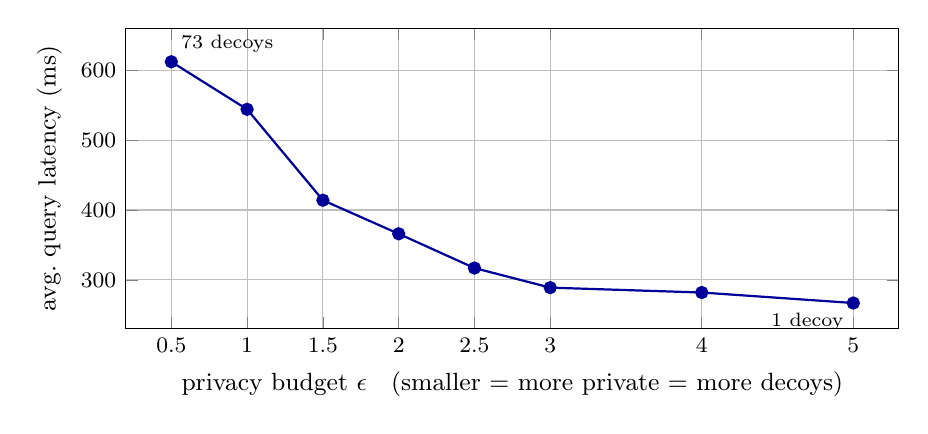
\begin{tikzpicture}
  \begin{axis}[
    width=0.94\linewidth, height=5.4cm,
    xlabel={privacy budget $\epsilon$ \; (smaller $=$ more private $=$ more decoys)},
    ylabel={avg.\ query latency (ms)},
    xmin=0.2, xmax=5.3, ymin=230, ymax=660,
    xtick={0.5,1,1.5,2,2.5,3,4,5},
    grid=major, tick label style={font=\footnotesize},
    label style={font=\small},
    every axis plot/.append style={thick},
    nodes near coords style={font=\scriptsize},
  ]
  \addplot[mark=*,color=blue!60!black] coordinates {
    (0.5,612)(1.0,544)(1.5,414)(2.0,366)(2.5,317)(3.0,289)(4.0,282)(5.0,267)
  };
  % decoy-count annotations at the two ends
  \node[font=\scriptsize,anchor=south west] at (axis cs:0.5,612) {73 decoys};
  \node[font=\scriptsize,anchor=north east] at (axis cs:5,267) {1 decoy};
  \end{axis}
  \end{tikzpicture}
  \caption{\opaque{}'s tunable-privacy knob, measured end-to-end on SIFT~1M
    (strict top-8, NC=128, m6i.2xlarge, 50 queries). Sweeping $\epsilon$ moves
    the decoy count from 73 ($\epsilon{=}0.5$, 612\,ms) to 1 ($\epsilon{=}5$,
    267\,ms); per-query distinguishability is bounded by $e^{\epsilon}$. Latency
    falls monotonically while Recall@10 stays flat at ${\approx}96\%$
    (the ${\pm}1.5$ pp wobble is build-to-build $k$-means variance, not a
    privacy cost---decoys never change which real clusters are fetched).
    Access-pattern privacy is bought purely with latency, not accuracy.}
  \label{fig:epssweep}
\end{figure}

% - SIFT 1M (128-d): 99.8% R@10 @ 357ms (PQ-M8-probe8); 100% @ 652ms (probe-16). 8 vCPU.
% - DBpedia 1M (1536-d ada-002): 92.4% R@10 @ 1.17s P50 (PQ-M48, RA=2, Memory). m6i.4xlarge.
% - Threshold overhead: ~0--10%.
% - Ablations: NC=128 vs 256 (256 is 60--67% slower --- rejected); PQ-M sweep;
%   RA=1 vs 2 at high-dim; eps sweep (latency-vs-privacy curve).

% ---------------------------------------------------------------------------
\section{Discussion, Limitations \& Future Work}
\label{sec:discussion}
% - Malicious-server hardening.
% - GPU-accelerated HE (open normalization mismatch).
% - PIR upgrade path (SimplePIR) to convert statistical -> cryptographic access privacy,
%   as an opt-in flag.
% - eps composition over long query streams.

% ---------------------------------------------------------------------------
\section{Conclusion}
\label{sec:conclusion}

\begin{thebibliography}{9}
\bibitem{compass} J.~Zhu, S.~Patel, M.~Zaharia, R.~A.~Popa.
  Compass: Encrypted Semantic Search with High Accuracy. \emph{OSDI}, 2025.
\bibitem{tiptoe} A.~Henzinger et al.
  Private Web Search with Tiptoe. \emph{SOSP}, 2023.
\bibitem{pacmann} Pacmann: Efficient Private Approximate Nearest-Neighbor
  Search. \emph{ICLR}, 2025. % TODO: full author list + exact title.
\bibitem{ppmi} Privacy-Preserving Million-scale Vector Search (PPMI).
  arXiv, 2025. % TODO: full author list + exact title.
\end{thebibliography}

\end{document}
